\documentclass[conference,a4paper]{IEEEtran}
\IEEEoverridecommandlockouts

\usepackage[utf8]{inputenc}
\usepackage[T1]{fontenc}
\usepackage{cite}
\usepackage{amsmath,amssymb,amsfonts}
\usepackage{algorithmic}
\usepackage{graphicx}
\usepackage{textcomp}
\usepackage{xcolor}
\usepackage{booktabs}
\usepackage{url}
\usepackage{hyperref}
\hypersetup{colorlinks=true, linkcolor=black, citecolor=black, urlcolor=blue}

\def\BibTeX{{\rm B\kern-.05em{\sc i\kern-.025em b}\kern-.08em
    T\kern-.1667em\lower.7ex\hbox{E}\kern-.125emX}}

\begin{document}

\title{Knowledge-Aware Evaluation for\\Legal Document Summarization}

\author{
\IEEEauthorblockN{Aditi Singh}
\IEEEauthorblockA{
\textit{E23CSEU1484}\\
\textit{Bennett University}
}
\and
\IEEEauthorblockN{Vaishnavi}
\IEEEauthorblockA{
\textit{E23CSEU1537}\\
\textit{Bennett University}
}
\and
\IEEEauthorblockN{Vasundhra Singh}
\IEEEauthorblockA{
\textit{E23CSEU1179}\\
\textit{Bennett University}
}
}

\maketitle

\begin{abstract}
Standard summarization metrics such as BLEU and ROUGE measure surface-level overlap and do not capture whether a legal summary preserves the case-defining \textit{intent} that determines the legal substance of a document. Mullick et al.~\cite{mullick2022} addressed this by introducing an Intent Metric based on exact-substring matching between annotated intent phrases and summary sentences. However, exact matching breaks down when summaries paraphrase. We extend their framework with two contributions: (1) a \textbf{Semantic Intent Metric (SIM)} that replaces binary substring matching with windowed cosine similarity over sentence-tuned MPNet embeddings, and (2) an \textbf{LLM-as-Judge} evaluator that scores intent preservation via a structured prompt. On 93 Indian legal documents across four case categories, SIM is the only automated metric showing a positive Spearman rank correlation with LLM-as-Judge ($\rho{=}{+}0.255$, $p{=}0.014$); BLEU, ROUGE-L, and the original exact-match Intent Metric all show weak negative correlations. The improvement is largest on cases involving abstract legal intent (Corruption, Land Dispute) and modest on cases dominated by concrete physical descriptors (Murder, Robbery), suggesting that semantic matching is most valuable when source phrases are likely to be paraphrased rather than copied.
\end{abstract}

\begin{IEEEkeywords}
legal summarization, evaluation metrics, intent extraction, semantic similarity, LLM-as-Judge
\end{IEEEkeywords}

\section{Introduction}

A practising lawyer typically reads through hundreds of pages of case proceedings to identify the substantive facts of a case. Court judgments routinely run to several thousand words, and Indian Supreme Court judgments average around 4{,}500 words \cite{mullick2022}. Automatic summarization can compress this material, but only if the resulting summaries preserve what makes the case legally meaningful: phrases such as \textit{``preparation to kill''}, \textit{``adverse possession''}, or \textit{``accepted illegal gratification''}. We refer to these as \textit{intent phrases}.

Existing summarization metrics struggle to evaluate intent preservation. Lexical metrics such as BLEU \cite{papineni2002bleu} and ROUGE \cite{lin2004rouge} count token overlap with a reference and ignore the legal weight of individual phrases. Embedding-based metrics such as BERTScore \cite{zhang2020bertscore} measure semantic similarity at the token or sentence level, but again do not target the specific phrases that define a case category. Mullick et al.~\cite{mullick2022} introduced an \textit{Intent Metric} that addresses this gap: given a document with annotated intent phrases, the metric reports the F1 of a substring match between phrases and summary sentences. Their Intent Metric correlated with human judgement better than BLEU or ROUGE on 101 Indian and 59 Australian legal documents.

The original Intent Metric has a structural limitation: substring matching is brittle to paraphrase. A summary that captures the meaning of \textit{``preparation to kill''} as \textit{``planned the killing''} receives zero credit. In legal summaries this is common: extractive summarizers select sentences whose wording differs from the annotated phrases, and abstractive summarizers can rephrase aggressively. Validating an evaluation framework against actual human ratings, as Mullick et al. did using crowd-sourced annotation, is also expensive and difficult to reproduce.

We make two contributions:

\begin{enumerate}
  \item We propose a \textbf{Semantic Intent Metric (SIM)} that replaces the binary substring match of \cite{mullick2022} with cosine similarity over MPNet \cite{song2020mpnet} sentence embeddings, computed over sliding word-windows inside each summary sentence. SIM identifies semantic equivalents of intent phrases that the original metric misses while preserving the same precision/recall/F1 framework.
  \item We integrate an \textbf{LLM-as-Judge} component \cite{liu2023geval, zheng2023judging} that prompts a small open-source language model to score intent preservation on a 1--5 Likert scale. This provides a reproducible, zero-cost reference signal that does not require crowd-sourced human ratings.
\end{enumerate}

We evaluate both contributions on the Indian-Data corpus released by \cite{mullick2022}: 93 documents annotated with intent phrases across four legal categories. SIM is the only automated metric that correlates positively and significantly with the LLM-as-Judge reference. The original Intent Metric, BLEU, and ROUGE-L all correlate negatively, indicating that they reward verbatim copying which does not reliably translate to preservation of legal intent.

\section{Related Work}

\subsection{Legal Document Summarization}
Approaches range from rule-based extractive systems such as LetSum \cite{farzindar2004letsum} and CaseSummarizer \cite{polsley2016casesummarizer}, to graphical-model methods using CRFs over rhetorical roles \cite{saravanan2006improving}, to transformer-based extractive \cite{miller2019leveraging} and abstractive \cite{beltagy2020longformer} models. Bhattacharya et al.~\cite{bhattacharya2019comparative} provide a comparative study on Indian Supreme Court judgments. Domain-specific encoders such as Legal-BERT \cite{chalkidis2020legal} have improved downstream performance on legal classification but were not originally designed for summarization evaluation.

\subsection{Summarization Evaluation}
Sai et al.~\cite{sai2020survey} survey evaluation metrics for natural language generation. Lexical metrics (BLEU, ROUGE, METEOR) measure surface overlap; embedding-based metrics (BERTScore, MoverScore, SMS \cite{clark2019sentence}) measure semantic similarity in a learned space. None of these are domain-aware: they treat all tokens equally, regardless of whether a token carries case-defining legal weight. Mullick et al.~\cite{mullick2022} introduced the first intent-aware evaluation framework for legal summarization, which is the direct baseline for our work.

\subsection{LLM-as-Judge}
Recent work uses large language models as automatic evaluators. G-Eval \cite{liu2023geval} prompts GPT-4 with structured rubrics; Zheng et al.~\cite{zheng2023judging} formalize the LLM-as-Judge paradigm and analyse its biases. We adopt this paradigm for legal summary evaluation, prompting a small open-source model with the source document, candidate summary, and annotated intent phrases.

\section{Methodology}

\subsection{Original Intent Metric}
We first reproduce the metric of Mullick et al.~\cite{mullick2022}. Given a document with $M$ annotated intent phrases $\{P_i\}_{i=1}^{M}$ and a candidate summary with $N$ sentences $\{O_j\}_{j=1}^{N}$, define a binary similarity:
\begin{equation}
s_{ij}^{\text{orig}} = \mathbb{1}\!\left[P_i \text{ is a substring of } O_j\right].
\end{equation}
Precision, recall, and F1 are computed as:
\begin{align}
P &= \frac{1}{N} \sum_{j=1}^{N} \mathbb{1}\!\left[\textstyle\sum_i s_{ij} > 0\right], \\
R &= \frac{1}{M} \sum_{i=1}^{M} \mathbb{1}\!\left[\textstyle\sum_j s_{ij} > 0\right], \\
F_1 &= \frac{2 P R}{P + R}.
\end{align}

\subsection{Semantic Intent Metric (SIM)}
We replace the substring match with semantic similarity. Let $\mathbf{e}(\cdot)$ denote a sentence-tuned embedding (we use \texttt{all-mpnet-base-v2} \cite{reimers2019sentencebert, song2020mpnet}). For each summary sentence $O_j$ we generate sliding word-windows $W_j^{(L)}$ of length $L$ approximately equal to the phrase length, with $50\%$ overlap. The semantic similarity score is:
\begin{equation}
s_{ij}^{\text{SIM}} = \mathbb{1}\!\left[\max_{w \in W_j^{(|P_i|)}} \cos\!\left(\mathbf{e}(P_i), \mathbf{e}(w)\right) \ge \tau \right].
\end{equation}
Two design choices matter. First, comparing a short phrase to an entire long summary sentence dilutes the cosine score because much of the sentence is unrelated context; matching against length-matched windows localises the comparison. Second, we use sentence-tuned MPNet rather than raw Legal-BERT because mean-pooled token embeddings of legal phrases cluster too tightly to discriminate between matches and non-matches in our pilot experiments. The threshold $\tau$ is selected by sweep (Section~\ref{sec:sim-threshold}).

\subsection{LLM-as-Judge}
We prompt an LLM with the source document, candidate summary, and annotated intent phrases, and ask it to rate intent preservation on a 1--5 Likert scale (1 = Very Poor, 5 = Excellent). The prompt is structured to require a JSON response with a numeric score and a one-sentence justification, parsed automatically. We use Qwen2.5-1.5B-Instruct \cite{qwen25} as a local, free, reproducible backend; the framework also supports Anthropic Claude and OpenAI GPT-4 backends via API.

\subsection{Evaluation Protocol}
We evaluate three metrics introduced above (Original Intent, SIM, LLM-Judge) alongside two lexical baselines (BLEU and ROUGE-L). Lexical baselines are computed against a pseudo-reference summary constructed from source sentences containing at least one annotated intent phrase. Following \cite{mullick2022}, we report Spearman rank correlation between the automated metrics and the reference signal (LLM-as-Judge in our setting; human ratings in \cite{mullick2022}).

\section{Experimental Setup}

\subsection{Dataset}
We use the Indian-Data corpus released by \cite{mullick2022}: 93 Indian Supreme Court / High Court judgments across four categories with manually annotated intent phrases. Statistics are summarised in Table~\ref{tab:dataset}.

\begin{table}[t]
\centering
\caption{Indian-Data statistics. Avg.~phrases is the average number of annotated intent phrases per document.}
\label{tab:dataset}
\small
\begin{tabular}{lcccc}
\toprule
Category & \# docs & avg.~words & avg.~sents & avg.~phrases \\
\midrule
Murder        & 30 & 1{,}560 & 149 & 18 \\
Land Dispute  & 25 & 2{,}461 & 196 & 22 \\
Robbery       & 21 & 1{,}907 & 162 & 17 \\
Corruption    & 17 & 2{,}542 & 197 & 16 \\
\midrule
\textbf{All}  & \textbf{93} & \textbf{2{,}023} & \textbf{173} & \textbf{18} \\
\bottomrule
\end{tabular}
\end{table}

\subsection{Summarization}
We generate extractive summaries using the BERT-based clustering method of Miller~\cite{miller2019leveraging}: sentences are encoded with \texttt{all-MiniLM-L6-v2}, clustered with $k$-means, and the sentence closest to each cluster centroid is selected. The number of clusters is set to $30\%$ of the source sentence count, matching the ratio used by \cite{mullick2022}.

\subsection{SIM Threshold Selection}
\label{sec:sim-threshold}

\begin{figure}[t]
\centering
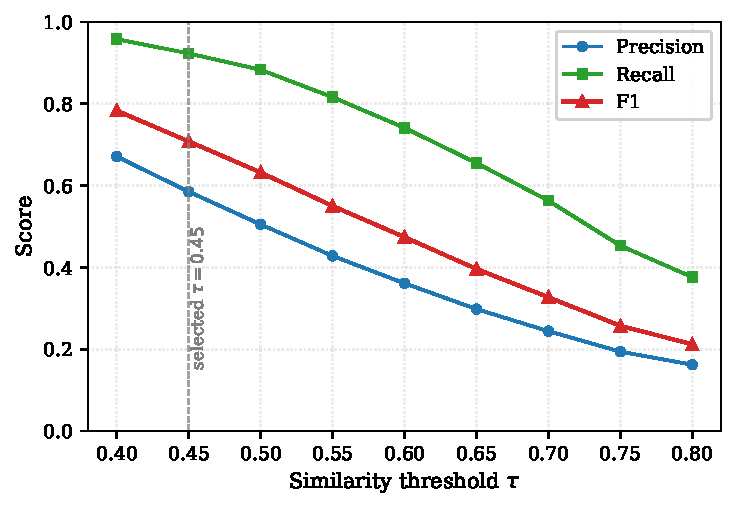
\includegraphics[width=\linewidth]{figures/fig_threshold_sweep.pdf}
\caption{SIM precision, recall, and F1 as a function of the cosine threshold $\tau$. Selected $\tau{=}0.45$ (dashed line) maximises F1 in the operating range $\tau \in [0.45, 0.70]$.}
\label{fig:threshold-sweep}
\end{figure}

We sweep $\tau \in \{0.40, 0.45, \ldots, 0.80\}$ and select the value maximising mean F1 in the range $[0.45, 0.70]$ where the metric is neither saturated (every match counted at low $\tau$) nor empty (no matches at high $\tau$). Figure~\ref{fig:threshold-sweep} shows the sweep. We select $\tau{=}0.45$, which gives mean precision $0.585$, mean recall $0.923$, and mean F1 $0.708$. We exclude $\tau{=}0.40$ from selection: at that value precision drops below $0.67$ while recall is near saturation, indicating over-permissive matching.

\subsection{Implementation}
All experiments run on a single Colab T4 GPU. SIM uses \texttt{all-mpnet-base-v2} (438MB). LLM-as-Judge uses \texttt{Qwen2.5-1.5B-Instruct} (3GB) loaded locally; no API access required. Total runtime for the 93-document evaluation is approximately 50 minutes. Code is released in a single Jupyter notebook for reproducibility.

\section{Results}

\subsection{Metric Averages}
Table~\ref{tab:averages} reports the mean of each metric across the 93 documents at $\tau{=}0.45$ for SIM.

\begin{table}[t]
\centering
\caption{Mean metric scores on Indian-Data ($n{=}93$).}
\label{tab:averages}
\small
\begin{tabular}{lc}
\toprule
Metric & Mean \\
\midrule
BLEU                            & 0.190 \\
ROUGE-L                         & 0.259 \\
Original Intent F1 \cite{mullick2022}    & 0.118 \\
\textbf{SIM F1 (ours)}          & \textbf{0.708} \\
LLM-as-Judge (1--5)             & 4.28 \\
\bottomrule
\end{tabular}
\end{table}

The Original Intent Metric scores low ($0.118$) because BERT-based extractive summarization rarely copies annotated intent phrases verbatim. SIM recovers most of this ``missing'' intent through semantic matching, scoring $0.708$, an absolute gain of $0.59$.

\subsection{Correlation with LLM-as-Judge}

\begin{table}[t]
\centering
\caption{Spearman rank correlation between automated metrics and LLM-as-Judge scores on Indian-Data ($n{=}93$). $^{*}$ indicates $p < 0.05$.}
\label{tab:correlation}
\small
\begin{tabular}{lcc}
\toprule
Metric & Spearman $\rho$ & $p$-value \\
\midrule
BLEU                       & $-0.173$ & $0.097$ \\
ROUGE-L                    & $-0.164$ & $0.116$ \\
Original Intent F1         & $-0.212$ & $0.041^{*}$ \\
\textbf{SIM F1 (ours)}     & $\mathbf{+0.255}$ & $\mathbf{0.014^{*}}$ \\
\bottomrule
\end{tabular}
\end{table}

Table~\ref{tab:correlation} reports the Spearman rank correlation between each automated metric and the LLM-as-Judge score. SIM is the only metric showing a significant positive correlation ($\rho{=}{+}0.255$, $p{=}0.014$). The original Intent Metric correlates significantly \textit{negatively} with the LLM-Judge ($\rho{=}{-}0.212$, $p{=}0.041$); BLEU and ROUGE-L show weak negative correlations.

\begin{figure}[t]
\centering
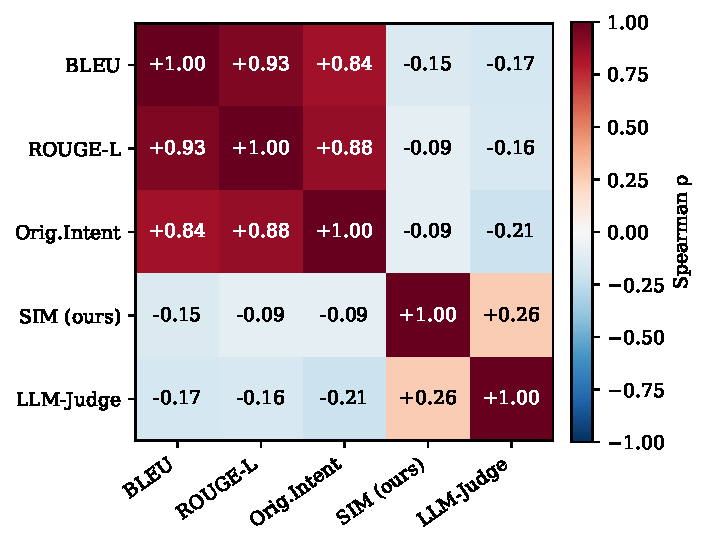
\includegraphics[width=\linewidth]{figures/fig_correlation_matrix.pdf}
\caption{Spearman rank correlation between all metric pairs on Indian-Data. Lexical metrics (BLEU, ROUGE-L, Original Intent) form one cluster; SIM and LLM-Judge form another.}
\label{fig:corr-matrix}
\end{figure}

Figure~\ref{fig:corr-matrix} visualises the full metric-vs-metric correlation matrix. BLEU, ROUGE-L, and Original Intent are tightly correlated with each other ($\rho{>}0.83$), reflecting that all three reward verbatim overlap with the source. SIM and LLM-Judge form a separate cluster: each correlates weakly negatively with the lexical group, and positively with each other. This suggests SIM and LLM-Judge measure a distinct property---semantic intent preservation---that is not captured by the lexical family.

\subsection{Per-Category Analysis}

\begin{figure}[t]
\centering
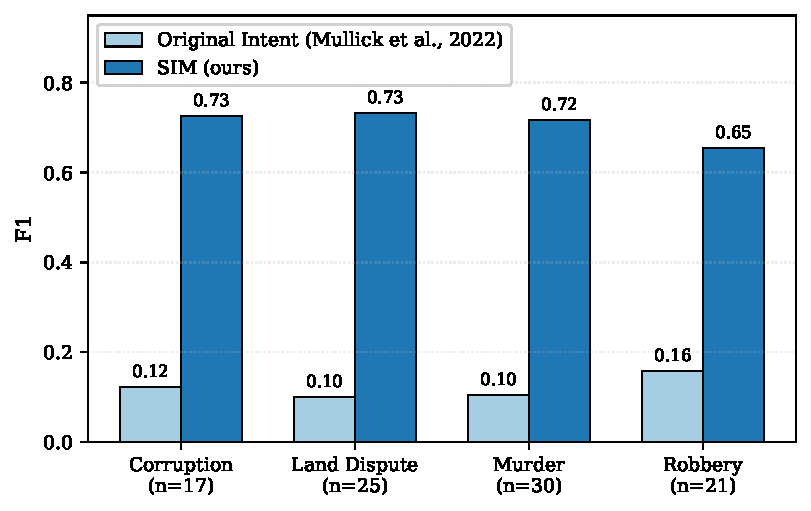
\includegraphics[width=\linewidth]{figures/fig_category_comparison.pdf}
\caption{Per-category mean F1: Original Intent vs.~SIM. SIM consistently recovers $0.5$--$0.6$ in absolute F1 across all categories.}
\label{fig:cat-bars}
\end{figure}

Figure~\ref{fig:cat-bars} compares per-category F1 between the original metric and SIM. The absolute gain is largest on Land Dispute ($+0.63$) and Murder ($+0.61$), and smallest on Robbery ($+0.50$). More informatively, Table~\ref{tab:per-cat-corr} reports the per-category Spearman correlation of SIM with LLM-Judge.

\begin{table}[t]
\centering
\caption{Per-category Spearman correlation between SIM and LLM-Judge. SIM is significantly positive on Corruption and Land Dispute. $^{*}$ indicates $p < 0.05$.}
\label{tab:per-cat-corr}
\small
\begin{tabular}{lcc}
\toprule
Category ($n$) & SIM $\rho$ & $p$-value \\
\midrule
Corruption (17)   & $+0.488$ & $0.047^{*}$ \\
Land Dispute (25) & $+0.464$ & $0.020^{*}$ \\
Murder (30)       & $+0.200$ & $0.289$ \\
Robbery (21)      & $-0.236$ & $0.303$ \\
\bottomrule
\end{tabular}
\end{table}

SIM is significantly positive on Corruption and Land Dispute, near zero on Murder, and weakly negative on Robbery. We interpret this as a consequence of intent phrase character: Corruption and Land Dispute phrases tend to be more abstract and legalistic (\textit{``accepted illegal gratification''}, \textit{``adverse possession''}), where summaries are likely to paraphrase. Murder and Robbery phrases are often concrete and physical (\textit{``stabbed with knife''}, \textit{``robbed articles''}), where exact-match and semantic-match agree more closely, leaving SIM with less ``room to add value''.

\subsection{SIM vs.~LLM-Judge Scatter}

\begin{figure}[t]
\centering
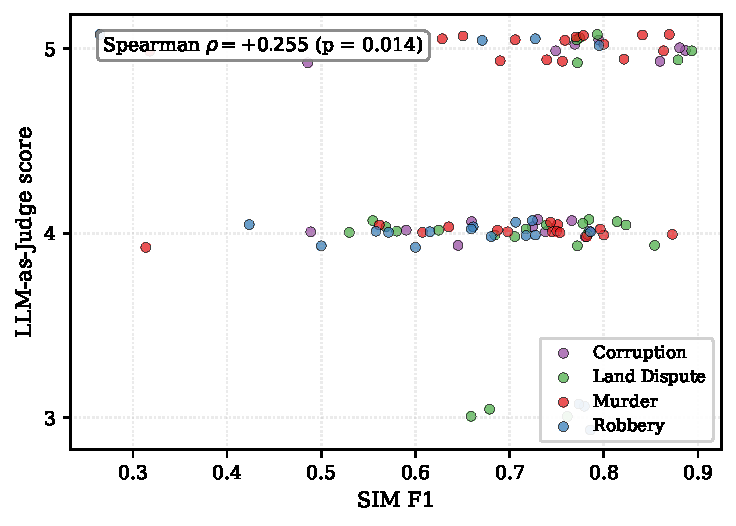
\includegraphics[width=\linewidth]{figures/fig_sim_vs_judge.pdf}
\caption{Per-document SIM F1 against LLM-as-Judge score, coloured by category. Vertical jitter is added to LLM scores (integers 3--5) for visibility.}
\label{fig:scatter}
\end{figure}

Figure~\ref{fig:scatter} shows the per-document scatter. Documents receiving an LLM-Judge score of 5 cluster at higher SIM F1 than those receiving 3 or 4, consistent with the positive Spearman correlation. The relationship is monotonic but noisy, reflecting the discreteness of the LLM-Judge scale and the heterogeneity of legal documents within each category.

\section{Discussion}

\subsection{Why Does the Original Intent Metric Correlate Negatively with LLM-Judge?}
This is the most surprising finding. We attribute it to the behaviour of the BERT extractive summarizer used in our experiments: it tends to select long, procedurally-rich sentences (e.g., headers, citations, court names) that happen to contain verbatim intent phrases as fragments. The original metric scores these summaries high because the substring is present, but the surrounding context is procedural noise that the LLM-Judge penalises. SIM, by contrast, requires \textit{semantic} similarity in a length-matched window, which discounts surrounding noise. Lexical metrics inherit the same bias as the original metric: they reward overlap with sentences that are intent-bearing-but-procedural, which the LLM does not view as good summaries.

\subsection{Where SIM Helps Most}
SIM's added value is concentrated on cases where intent is encoded in legalistic abstractions rather than physical descriptors. This pattern aligns with intuition about the corpus: legal disputes over corruption or property rights are framed in interpretive language that admits many surface forms, whereas violent-crime descriptions tend to use a more standardised concrete vocabulary.

\subsection{Why a Sentence-Tuned Encoder Rather than Legal-BERT}
In a pilot, we compared mean-pooled \texttt{nlpaueb/legal-bert-base-uncased} embeddings against \texttt{all-mpnet-base-v2}. Raw Legal-BERT mean-pooled embeddings of legal phrases consistently fell within a narrow cosine band ($\sim 0.6$--$0.7$) regardless of whether the pair was a true match or merely topical, giving a poor decision boundary. MPNet, contrastively pretrained on sentence-pair similarity, separates matches from non-matches with a wider gap. We therefore use MPNet despite Legal-BERT's domain familiarity.

\section{Limitations}

\textbf{Reference signal is an LLM, not human ratings.} The original \cite{mullick2022} framework used crowd-sourced human ratings on the Appen platform. Our reference signal is a small open-source LLM (Qwen2.5-1.5B). LLM-as-Judge scores can systematically diverge from expert human judgement \cite{zheng2023judging}, and our positive correlation between SIM and LLM-Judge could in part reflect shared inductive biases between MPNet and Qwen rather than alignment with human preference. Validation against expert human annotation, in particular by lawyers, is left to future work.

\textbf{Single corpus.} We evaluate only on Indian-Data (93 documents). Generalisation to the Australian-Data corpus released by \cite{mullick2022}, or to legal corpora from other jurisdictions, has not been verified.

\textbf{Single summarizer.} All experiments use the BERT-extractive summarizer of Miller~\cite{miller2019leveraging}. The relative ranking of metrics may differ for graphical-CRF \cite{saravanan2006improving}, abstractive \cite{beltagy2020longformer}, or LLM-based summarizers.

\textbf{Threshold selection.} The SIM threshold $\tau{=}0.45$ is selected on the same 93 documents on which we report results, raising the possibility of mild over-fitting. A held-out tuning set would be preferable; we did not split the data given its small size.

\textbf{Statistical power.} With $n{=}93$, the per-corpus Spearman correlations are significant at $p{<}0.05$ but the per-category breakdown ($n{=}17$--$30$) has low power, particularly for Murder and Robbery.

\section{Conclusion}

We extended the intent-aware evaluation framework of Mullick et al.~\cite{mullick2022} along two axes: (1) replacing exact-substring matching with windowed cosine similarity over MPNet embeddings (SIM), and (2) integrating an LLM-as-Judge reference signal. On 93 Indian legal documents, SIM is the only automated metric that correlates positively and significantly with LLM-Judge scores ($\rho{=}{+}0.255$, $p{=}0.014$); BLEU, ROUGE-L, and the original Intent Metric correlate weakly negatively. The improvement is concentrated on Corruption and Land Dispute cases, where intent phrases admit more paraphrase. SIM is free, reproducible, and computable in $\sim$10 minutes on a free-tier GPU, suggesting it is suitable as a deployment metric where access to expert human raters is impractical.

\begin{thebibliography}{00}

\bibitem{beltagy2020longformer}
I.~Beltagy, M.~E. Peters, and A.~Cohan, ``Longformer: The long-document transformer,'' \textit{arXiv:2004.05150}, 2020.

\bibitem{bhattacharya2019comparative}
P.~Bhattacharya, K.~Hiware, S.~Rajgaria, N.~Pochhi, K.~Ghosh, and S.~Ghosh, ``A comparative study of summarization algorithms applied to legal case judgments,'' in \textit{Proc. ECIR}, 2019, pp.~413--428.

\bibitem{chalkidis2020legal}
I.~Chalkidis, M.~Fergadiotis, P.~Malakasiotis, N.~Aletras, and I.~Androutsopoulos, ``LEGAL-BERT: The Muppets straight out of Law School,'' in \textit{Findings of EMNLP}, 2020.

\bibitem{clark2019sentence}
E.~Clark, A.~Celikyilmaz, and N.~A. Smith, ``Sentence Mover's Similarity: Automatic evaluation for multi-sentence texts,'' in \textit{Proc. ACL}, 2019.

\bibitem{farzindar2004letsum}
A.~Farzindar and G.~Lapalme, ``LetSum, a text summarization system in law field,'' in \textit{The Face of Text}, 2004, pp.~27--36.

\bibitem{lin2004rouge}
C.-Y. Lin, ``ROUGE: A package for automatic evaluation of summaries,'' in \textit{Text Summarization Branches Out}, 2004.

\bibitem{liu2023geval}
Y.~Liu, D.~Iter, Y.~Xu, S.~Wang, R.~Xu, and C.~Zhu, ``G-Eval: NLG evaluation using GPT-4 with better human alignment,'' in \textit{Proc. EMNLP}, 2023.

\bibitem{miller2019leveraging}
D.~Miller, ``Leveraging BERT for extractive text summarization on lectures,'' \textit{arXiv:1906.04165}, 2019.

\bibitem{mullick2022}
A.~Mullick, A.~Nandy, M.~N. Kapadnis, S.~Patnaik, R.~Raghav, and R.~Kar, ``An evaluation framework for legal document summarization,'' in \textit{Proc. LREC}, 2022.

\bibitem{papineni2002bleu}
K.~Papineni, S.~Roukos, T.~Ward, and W.-J. Zhu, ``BLEU: a method for automatic evaluation of machine translation,'' in \textit{Proc. ACL}, 2002, pp.~311--318.

\bibitem{polsley2016casesummarizer}
S.~Polsley, P.~Jhunjhunwala, and R.~Huang, ``CaseSummarizer: A system for automated summarization of legal texts,'' in \textit{Proc. COLING Demonstrations}, 2016, pp.~258--262.

\bibitem{qwen25}
Qwen Team, ``Qwen2.5: A party of foundation models,'' \url{https://qwenlm.github.io/blog/qwen2.5/}, 2024.

\bibitem{reimers2019sentencebert}
N.~Reimers and I.~Gurevych, ``Sentence-BERT: Sentence embeddings using Siamese BERT-Networks,'' in \textit{Proc. EMNLP}, 2019.

\bibitem{sai2020survey}
A.~B. Sai, A.~K. Mohankumar, and M.~M. Khapra, ``A survey of evaluation metrics used for NLG systems,'' \textit{arXiv:2008.12009}, 2020.

\bibitem{saravanan2006improving}
M.~Saravanan, B.~Ravindran, and S.~Raman, ``Improving legal document summarization using graphical models,'' \textit{Frontiers in AI and Applications}, vol.~152, p.~51, 2006.

\bibitem{song2020mpnet}
K.~Song, X.~Tan, T.~Qin, J.~Lu, and T.-Y. Liu, ``MPNet: Masked and permuted pre-training for language understanding,'' in \textit{Proc. NeurIPS}, 2020.

\bibitem{zhang2020bertscore}
T.~Zhang, V.~Kishore, F.~Wu, K.~Q. Weinberger, and Y.~Artzi, ``BERTScore: Evaluating text generation with BERT,'' in \textit{Proc. ICLR}, 2020.

\bibitem{zheng2023judging}
L.~Zheng, W.-L. Chiang, Y.~Sheng, et~al., ``Judging LLM-as-a-Judge with MT-Bench and Chatbot Arena,'' in \textit{Proc. NeurIPS Datasets and Benchmarks}, 2023.

\end{thebibliography}

\end{document}
